\documentclass[t, aspectratio=169]{beamer}
\usepackage{amsmath,amsfonts,amsthm,amstext,amssymb, xcolor, tikz, pgf, mathrsfs, polynom, pifont, tabto}

% ----------------------------------------------------------
% Theme Setup

% Use Metropolis Theme
\usetheme[numbering=fraction]{metropolis}
\setbeamertemplate{blocks}[rounded][shadow=false]
\makeatletter
\setlength{\metropolis@titleseparator@linewidth}{1pt}
\makeatother

% Define Colors
\definecolor{chargerblue}{HTML}{002764}
\definecolor{chargerred}{HTML}{e02034}
\definecolor{bggray}{HTML}{d0d3d4}

% Set Colors
\setbeamercolor{title}{fg=chargerblue}
\setbeamercolor{background canvas}{bg=white}
\setbeamercolor{title separator}{fg=chargerred}
\setbeamercolor{structure}{fg=chargerblue}
\setbeamercolor{frametitle}{fg=white, bg=chargerblue}
\setbeamercolor*{normal text}{fg=chargerblue}
\setbeamercolor*{block body}{bg=bggray}
\setbeamercolor*{block title}{bg=chargerblue, fg=white}
% ----------------------------------------------------------

% ----------------------------------------------------------
% Custom Definitions, Commands, Environments, etc.

% Sets of numbers
\def\R{\mathbb{R}} % The reals
\def\N{\mathbb{N}} % The naturals
\def\Z{\mathbb{Z}} % The integers
\def\Q{\mathbb{Q}} % The rationals

% Blank space
\newcommand{\blank}[1]{\underline{\hspace{#1}}} % Blank space

% Change font colors
\newcommand{\cyan}[1]{{\color{cyan}{#1}}} % Changes font to cyan
\newcommand{\red}[1]{{\color{red}{#1}}} % Changes font to red
\newcommand{\magenta}[1]{{\color{magenta}{#1}}} % Changes font to magenta
\newcommand{\orange}[1]{{\color{orange}{#1}}} % Changes font to orange
\newcommand{\yellow}[1]{{\color{yellow}{#1}}} % Changes font to yellow
\newcommand{\violet}[1]{{\color{violet}{#1}}} % Changes font to violet
\newcommand{\green}[1]{{\color{green}{#1}}} % Changes font to green
\newcommand{\blue}[1]{{\color{blue}{#1}}} % Changes font to blue
\newcommand{\white}[1]{{\color{white}{#1}}} % Changes font to white

% Fitted inclusion symbols
\newcommand{\fp}[1]{\left({#1}\right)} % Fitted parentheses around content
\newcommand{\fb}[1]{\left[{#1}\right]} % Fitted brackets
\newcommand{\lhoi}[1]{\left({#1}\right]} % Left half-open interval
\newcommand{\rhoi}[1]{\left[{#1}\right)} % Right half-open interval
\newcommand{\set}[1]{\left\{{#1}\right\}} % Fitted braces (useful for sets)
\newcommand{\av}[1]{\left|{#1}\right|} % Fitted absolute value bars

% Augmented Matrix Environment
\newenvironment{amatrix}[1]{%
	\left[\begin{array}{@{}*{#1}{c}|c@{}}
	}{%
	\end{array}\right]
}

% Miscellaneous
\def\then{\Rightarrow}
\def\to{\rightarrow}
\def\d{^{\circ}}
\newcommand{\?}{\stackrel{?}{=}}
\newcommand{\cmark}{\text{ \ding{51}}}
\newcommand{\xmark}{\text{ \ding{55}}}

% Coordinate Plane (Four-Quadrant)
\def\coordplane {
	\begin{tikzpicture}        \draw[step=0.25cm,black,very thin,opacity=0.25] (-2.5cm, -2.5cm) grid (2.5cm, 2.5cm);
		\draw[<->,thick,black] (-2.5cm, 0) -- (2.5cm, 0) node[anchor=north west,pos=0.94,font=\scriptsize]{$x$};
		\draw[<->,thick,black] (0,-2.5cm) -- (0, 2.5cm) node[anchor=south east,font=\scriptsize,pos=0.94]{$y$};
	\end{tikzpicture}
}

% Coordinate Plane (One-Quadrant)
\def\onequad {
	\begin{tikzpicture}
		\draw[step=0.25cm, black, very thin, opacity=0.25] (0,0) grid (7.5cm,5cm);
		\draw[->, thick, black] (0,0) -- (7.5cm, 0) node[anchor=north west,font=\scriptsize,pos=0.94]{$x$};
		\draw[->, black, thick] (0,0) -- (0,5cm) node[anchor=south east,font=\scriptsize,pos=0.94]{$y$};
	\end{tikzpicture}
}
% ----------------------------------------------------------

% ----------------------------------------------------------
% Presentation Information
\title[7-3]{Confidence Intervals and Sample Size for Proportions}
\subtitle{Section 7-3}
\author{Jacob Ayers}
\institute{Lesson \#23}
\date{MAT 110}
% ----------------------------------------------------------

\begin{document}
	
	% Slide 1 (Title Slide)
	\begin{frame}
		\titlepage
	\end{frame}
	
	% Slide 2 (Objectives)
	\begin{frame}{Objectives}
		\begin{itemize}
			\item Find the confidence interval for a proportion.
			\item Determine minimum sample size for finding a confidence interval for a proportion.
		\end{itemize}
	\end{frame}

	\begin{frame}{Confidence Intervals for Proportions}
		Many statistical studies aim to find the proportion (aka percentage) of a population with certain characteristics. \pause
		
		Examples: \begin{itemize}
			\item Polls before elections \pause
			\item Opinion surveys on cell phones \pause
			\item Determining popular baby names \pause
		\end{itemize}
	
		As with sample means, the proportions found in samples will not match the actual proportion population. \pause
		
		We instead use an interval estimate (aka a confidence interval).
	\end{frame}

	\begin{frame}{Symbols Used in Proportion Notation}
		We use $p$ to denote the \textit{population proportion} \pause
		
		$\hat{p}$ (read ``p hat") is used to represent the \textit{sample proportion} \pause
		
		When computing a sample proportion, $\hat{p} = \dfrac{X}{n}$; $X$ is the number sampled that have the given characteristic, and $n$ is the total number sampled. \pause
		
		$\hat{q} = \dfrac{n - X}{n} = 1 - \hat{p}$ is the proportion of the sample that doesn't have the given characteristic.
		
		Example: In a survey, 55 out of 120 workers said their job was stressful. \pause
		
		In this case, $X = 55$, \pause $n = 120$, \pause $\hat{p} = \dfrac{55}{120} \approx 0.4583$, \pause and $\hat{q} = \dfrac{120 - 55}{120} = 1 - \hat{p} \approx 0.5417$
	\end{frame}

	\begin{frame}{Finding $\hat{p}$ and $\hat{q}$}
		A random sample of 150 assault victims in a large city found that 45 took so self-protection actions against the criminal. Find $\hat{p}$ and $\hat{q}$, where $\hat{p}$ is the proportion of victims who took no self-protection action against the criminal. \pause
		
		$n = 150$ \pause \\
		45 took no action, so $X = 45$ \pause
		
		Thus, $\hat{p} = \dfrac{45}{150} = 0.3$. \pause
		
		$\hat{q} = 1 - 0.3 = 0.7$
	\end{frame}

	\begin{frame}{Confidence Intervals for Proportion}
		As with confidence intervals for the mean, we need to find the margin of error. For proportions, we use the standard normal ($z$) table. \pause
		
		The margin of error is $E = z_{\alpha / 2}\sqrt{\dfrac{\hat{p}\hat{q}}{n}}$ \pause
		
		The formula for the confidence interval is $$\hat{p} - z_{\alpha / 2}\sqrt{\dfrac{\hat{p}\hat{q}}{n}} < p < \hat{p} + z_{\alpha / 2}\sqrt{\dfrac{\hat{p}\hat{q}}{n}}$$ \pause
		Assumptions for Confidence Intervals for Proportions: \begin{enumerate}[1)]
			\item $n\hat{p} \geq 5$, $n\hat{q} \geq 5$ \pause
			\item Random sample
			\item Distribution is binomial
		\end{enumerate}
	\end{frame}

	\begin{frame}{Confidence Intervals for Proportion}
		The procedure for constructing a confidence interval for a proportion is: \begin{enumerate}[1)]
			\item Find $\hat{p}$ and $\hat{q}$. \pause
			\item Make sure the assumptions hold. \pause
			\item Calculate $\sqrt{\dfrac{\hat{p}\hat{q}}{n}}$; store this value. \pause
			\item Look up $z_{\alpha / 2}$ (remember: 90\% is 1.65, 95\% is 1.96, 99\% is 2.58). \pause
			\item Use the formula $$\hat{p} - z_{\alpha / 2}\sqrt{\dfrac{\hat{p}\hat{q}}{n}} < p < \hat{p} + z_{\alpha / 2}\sqrt{\dfrac{\hat{p}\hat{q}}{n}}$$ to find the lower and upper limits; write the interval.
		\end{enumerate}
	\end{frame}

	\begin{frame}{Confidence Intervals for Proportion}
		A survey of 1000 U.S. adults found that 33\% of people said that they would get no work done on Cyber Monday since they would spend all day shopping online. Find the 95\% confidence interval of the true proportion. \pause
		
		1) $\hat{p} = 0.33$; $\hat{q} = 1 - 0.33 = 0.67$. \pause \\
		2) Assumptions hold. \pause \\
		3) Using a calculator, $\sqrt{\dfrac{\hat{p}\hat{q}}{n}} = \sqrt{\dfrac{0.33(0.67)}{1000}} \approx 0.0148694317$. \pause \\
		4) 95\% confidence $\then$ $z_{\alpha / 2} = 1.96$ \pause
		
		5) Lower Limit for CI: $0.33 - 1.96(0.0149) \approx 0.301$ \pause \\
		Upper Limit for CI: $0.33 + 1.96(0.0149) \approx 0.359$ \pause
		
		The confidence interval is $0.301 < p < 0.359$\pause; we are 95\% confident that the population proportion is between 30.1\% and 35.9\%
	\end{frame}

	\begin{frame}{Confidence Intervals for Proportion}
		A survey of 50 students in grades 4 through 12 found 68\% have classroom Wi-Fi access. Find the 99\% confidence interval of the population proportion. \pause
		
		1) $\hat{p} = 0.68$; $\hat{q} = 1 - 0.68 = 0.32$ \pause \\
		2) Assumptions hold. \pause \\
		3) Using a calculator, $\sqrt{\dfrac{\hat{p}\hat{q}}{n}} = \sqrt{\dfrac{0.68(0.32)}{50}} \approx 0.06596969$. \pause \\
		4) 99\% confidence $\then$ $z_{\alpha_2} = 2.58$. \pause
		
		5) Lower Limit for CI: $0.68 - 2.58(0.0660) \approx 0.510$ \pause \\
		Upper Limit for CI: $0.68 + 2.58(0.0660) \approx 0.850$ \pause
		
		The confidence interval is: $0.510 < p < 0.850$
	\end{frame}

	\begin{frame}{Sample Size for Proportions}
		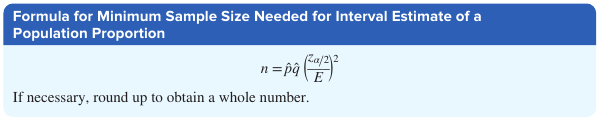
\includegraphics[width=\textwidth]{sample.png} \pause
		
		If $\hat{p}$ is known, use it. If $\hat{p}$ is not known, use $\hat{p} = 0.5$. \pause
		
		Reason: This maximizes the value of $\hat{p}\hat{q}$, which gives the largest possible value of $n$ (i.e. it's conservative). \pause
		
		Downside: Can lead to larger sample size that is actually necessary.
	\end{frame}

	\begin{frame}{Sample Size for Proportions}
		A researcher wishes to estimate, with 95\% confidence, the proportion of people who did not have a landline phone. A previous study shows that 40\% of those interviewed did not have a landline phone. The researcher wishes to be accurate within 2\% of the true proportion. Find the minimum required sample size.
		\begin{flalign*}
			\onslide<2->{n &= \hat{p}\hat{q}\fp{\dfrac{z_{\alpha/2}}{E}}^2 & \\}
			\onslide<3->{&= 0.4(0.6)\fp{\dfrac{1.96}{0.02}}^2 & \\}
			\onslide<4->{&= 0.24(98)^2 & \\}
			\onslide<5->{&= 2304.96}
		\end{flalign*}
		\onslide<6->{A sample size of 2305 is required.}
	\end{frame}

	\begin{frame}{Sample Size for Proportions}
		It is believed that 25\% of U.S. homes have a direct satellite television receiver. How large a sample is necessary to estimate the true population proportion of homes that do with 95\% confidence and with 3 percentage points?
		\begin{flalign*}
			\onslide<2->{n &= \hat{p}\hat{q}\fp{\dfrac{z_{\alpha/2}}{E}}^2 & \\}
			\onslide<3->{&= 0.25(0.75)\fp{\dfrac{1.96}{0.03}}^2 & \\}
			\onslide<4->{&= 0.1875(65.33)^2 & \\}
			\onslide<5->{&\approx 800.33}
		\end{flalign*}
		\onslide<6->{801 homes should be surveyed.}
	\end{frame}

	\begin{frame}{Sample Size for Proportions}
		Rework the following example if nothing is known about the proportion. \pause
		
		\onslide<2->{Since nothing is known, use $\hat{p} = 0.5$ (so $\hat{q} = 0.5$ as well).}
		\begin{flalign*}
			\onslide<3->{n &= \hat{p}\hat{q}\fp{\dfrac{z_{\alpha/2}}{E}}^2 & \\}
			\onslide<4->{&= 0.5(0.5)\fp{\dfrac{1.96}{0.03}}^2 & \\}
			\onslide<5->{&= 0.25(65.33)^2 & \\}
			\onslide<6->{&\approx 1067.11}
		\end{flalign*}
		\onslide<7->{1068 homes should be surveyed.}
	\end{frame}

	\begin{frame}{Next Steps}
		\begin{itemize}
			\item Prepare for and take Midterm 2 \begin{itemize}
				\item Study Guide posted in Week 13 section
				\item Will take next Wednesday
			\end{itemize}
			\item Complete Assignment 11
			\item Begin Module \#14 \begin{itemize}
				\item Read 8-1
				\item Watch Video Lesson \#24
			\end{itemize}
		\end{itemize}
	
		\vfill
		
		Thanks for watching!
	\end{frame}
	
\end{document}